\subsection{Tiefenwahrnehmung des Menschen}\label{subsec:depth-percept}
Um zu verstehen, wie 3D-Medien kodiert werden k\"onnen, ist es zun\"achst wichtig zu verstehen, wie die Tiefenwahrnehmung
beim Menschen funktioniert.
Wir unterscheiden zwischen \textit{monokularen} und \textit{binokularen} Faktoren.
Monokulare Faktoren sind von nur einer Perspektive (Auge oder Kameralinse) abh\"angig.
Dazu z\"ahlen unter anderem\cite{depth-perception}:
\begin{itemize}
    \item Bewegungsparallaxe
    \item absolute/relative/vertraute Gr\"oße
    \item Verdeckung naher Objekte durch ferne Objekte
    \item Wahrnehmung dreidimensionaler Form durch Licht und Schatten
    \item Tiefensch\"arfe
\end{itemize}
Diese Effekte sind allesamt in nur einem einzelnen Datenstrom enkodierbar und essentiell f\"ur ein immersives Bild.

\noindent\newline Mehrere Datenstr\"ome werden hingegen f\"ur binokulare Faktoren ben\"otigt.
Hierzu z\"ahlt die Parallaxe zwischen dem linken und dem rechten Auge, sprich der Unterschied dieser zwei Perspektiven.
Objekte die hierbei n\"aher zum Betrachter liegen, werden unterschiedlicher von den Augen wahrgenommen, weiter entferntere
Objekte hingegen \"ahnlicher.
Dieser Faktor erlaubt eine \textit{echte} Tiefenwahrnehmung bis zu 10m.\cite{depth-perception}
Weiterhin wird Tiefe durch die Konvergenz der Blickachsen des Betrachters wahrgenommen.
Um besonders nahe gelegene Objekte zu betrachten, muss der Mensch seine Augen leicht nach innen drehen um das Objekt
scharf zu sehen, was dem Gehirn wiederhin erm\"oglicht, Tiefe aus dieser Konvergenz zu interpretieren.

\noindent\newline Da das \"Andern der Blickachsen eines Zuschauers ohne Gewalt nicht m\"oglich ist, bleibt somit die
Parallaxe der entscheidende, zu reproduzierende Faktor um Videos mit 3D-Effekt zu erzeugen.


\subsection{Begriffskl\"arungen zum Thema Video}\label{subsec:video-terms}
\subsubsection{Codec}
Der Begriff Codec setzt sich aus den englischen W\"ortern \textbf{co}der (Kodierer) / \textbf{dec}oder (Dekodierer)
zusammen\cite{codec} und ist ein Algorithmenpaar bestehend aus den genannten Teilen.
Er wird jedoch vor allem im Themenbereich Medien eingesetzt um Audio- und Videostandards wie \texttt{H.264} zu
bezeichnen.

\noindent\newline So ist z.B. \texttt{H.264/AVC} ein Codec, \texttt{MP4} hingegen ein Containerformat, sprich ein Dateiformat welches
die kodierten Datenstr\"ome eines Codecs enth\"alt.

\noindent\newline Die Begriffe \textit{encoder} und \textit{decoder} hingegen werden f\"ur konkrete Programme zum
Kodieren oder Dekodieren der Datenstr\"ome eines Codecs verwendet.
So ist z.B. \textt{x264}\cite{x264} ein \textit{encoder} f\"ur den Codec \texttt{H.264}

\subsection{H.264}\label{subsec:h.264}
H.264 ist ein Codec, welcher 2003\cite{h264} durch die VCEG (\textit{Video Coding Experts Group}) und MPEG
(\textit{Moving Pictures Expert Group}) als \textit{MPEG Part 10} standardisiert wurde.
Er wird auch als AVC (\textit{Advanced Video Codec}) bezeichnet.

\noindent\newline H.264 unterst\"utzt sowohl \textit{Intra-Frame-Kompression}, die Kompression von Daten innerhalb eines Rahmens sowie
\textit{Inter-Frame-Kompression}, die Kompression zwischen mehreren Rahmen.

\noindent\newline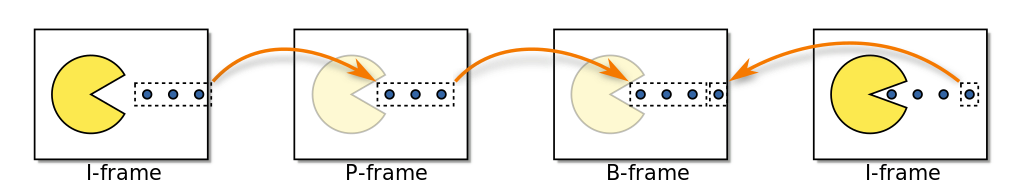
\includegraphics[width=\textwidth]{../img/frames}

\noindent\newline Kompression von Videodaten erfolgt in sogenannten \textit{Macrobl\"ocken}.
Hierbei handelt is sich um 4x4 bis 16x16 gro{\ss}e Bl\"ocke von Pixeln.

%\paragraph{Outline}
%\section*{8 Literaturverzeichnis}\label{sec:bibliography}
%Section~\ref{sec:previous work} gives account of previous work.
%Our new and exciting results are described in Section~\ref{sec:results}.
%Finally, Section~\ref{sec:conclusions} gives the conclusions.
%    \section{Previous work}\label{sec:previous work}
%    A much longer \LaTeXe{} example was written by Gil~\cite{Gil:02}.

